\section{Benchmarks}\label{bench}
To demonstrate the feasibility of our protocol, as well as validate the performance estimates we have referenced in the preceding sections of this document, we have undertaken a series of experiments to quantify the variety of behaviors related to our protocol. These measurements have been used to classify the headline performance estimates previously referred to as throughout (i.e. TPS) and transaction finality (i.e. finality), as well as some less consequential discoveries of note.

\subsection{Methods}\label{bench:met}
We would like to preface the coming disclosure of \textit{Blossom} benchmarking with several statements clarifying the context of our experiments, as well as provide the reader with some reasonable expectations one must hold when analyzing the data. We believe these acknowledgments to be necessary, as there has been an observed behavior among industry members to purport performance benchmarking as “real world" performance, without much credence to the true circumstances with which the authors collected said measurements. 

With that being said, we would like to clarify all benchmarks disclosed in this document were collected in the AWS cloud, with a testing environment similar to what may be considered sterile laboratory conditions. When a statement is made, we will make sure to notate the relevant infrastructure as well as the observed hardware utilization of said systems. Regarding the tolerances of our testing, we recognize that all nodes in the simulation operated within a trusted environment, and as such are not required to additionally manage the accessory behaviors required of an active network member. As we cannot quantify the ‘noise’ associated with the real-world operation, we would like to clarify, unless otherwise stated, the measurements in this document are intended to represent network performance in ideal conditions. For this reason, despite any specific performance figure we reference in this document, we would like to clarify our greatest innovation being \textit{scalable performance} (e.g. as the network increases in membership, the performance also increases).

To efficiently scale our network simulation across environments, we deployed blossom nodes using a container architecture, implementing Kubernetes to manage the orchestration of the associated distributed infrastructure \cite{burns2022kubernetes}. Each instance of the application was maintained as a replica service, with a permissioned address limiting communication to network members.  Given nodes operate as replica devices without the need to add or remove peers to or from the network, following cluster deployment nodes were required to log with a centralized Redis database (DB) \cite{carlson2013redis}. Nodes, expecting to maintain a ledger of $n$ peers, would then query the DB until they had stored the credentials for the entire network. For the release of \textit{Blossom} we recognize that such centralized infrastructure is non-viable, and intend on implementing a distributed hash table (DHT), such as Kademlia \cite{Maymounkov2002-in}, or a similar service to facilitate the decentralized addition and removal of nodes. However, for the purposes of our testing, we do not expect these approaches to return different results by a statistically significant margin.

To manage the undertaking of our simulation, many of the variables we have discussed throughout this document (network size, quorum size, block size, signature scheme, etc) are passed to nodes using environment variables at deployment. This allows us to easily initialize network simulations of variable size while guaranteeing no resources are utilized for non-relevant nodes. With the network successfully initialized, we may then begin sending requests to the network via a client. These requests are formatted as regular \texttt{HTTP messages} and allow for nodes to \texttt{GET} some network information from a node, or \texttt{POST} new transactions to a node. To undergo our testing of transaction throughput and finality we focused on \texttt{POST} requests, deploying specialized clients with the ability to create simulated transactions for the network to process. To limit any bottlenecks associated with any single client, nodes are designed to handle parallel communication, thus we are able to deploy more than one (1) client per network node if necessary; however, across our testing, we implemented the standard ratio of one (1) client for every six (6) nodes.

To better understand the scalability of \textit{Blossom} we have incorporated four (4) variables for our testing which may be strategically modulated to isolate the protocol’s unique limiting factors. Those variables include instance type (i.e. node \texttt{CPU} and \texttt{RAM}), node locations (i.e. colocated or globally distributed), signature verification, and network size.

\subsection{Results}\label{bench:res}
The network sizes we implemented as part of this experiment utilized the minimum quorum size $q$ of Blossom, with the number of nodes increasing at an exponential rate from the base value of $q$ (\(n = q^{[1:4]}\)). For deployment purposes, we have limited the largest number of nodes we test to \(n=1296\), with the variety of instances similarly limited, with a minimum resource allocation of about one (1) \texttt{vCPU} and maximum resource allocation of about eight (8) \texttt{vCPU} per node. For reference, the common threshold of decentralization for a network is 1,000 nodes.

The following figures (\textit{Figure} \ref{fig:test_tps}, \textit{Figure} \ref{fig:test_fin}, and \textit{Figure} \ref{fig:test_tx}) represent the data collected when all network members (nodes) are flooded with a surplus number of transactions, with the total cumulative number of transactions processed by the network equalling more than five (5) million. Due to our unique network architecture, and effective block cap, each node is only able to distribute a maximum of 1,000 transactions each epoch, thus the number of transactions distributed each epoch ($T$) is a function of the number of nodes (\(T=1000n\)).

Due to the nature of this test (over-saturating the network with transactions) we expect to see finality times increase with the number of active nodes, while (due to the need to complete compute-heavy tasks, such as that of signature verification, and our ability to process this task in a parallelized manner) we expect that as the number of \texttt{CPU} cores utilized by each node increase, the finality time of each epoch will decrease, thus increasing the overall throughput of the network. We expect these changes in performance to be linearly correlated with the change in compute resources (\texttt{CPU}) available to each node, up until some threshold is met.



\begin{figure}[h!]
    \centering
    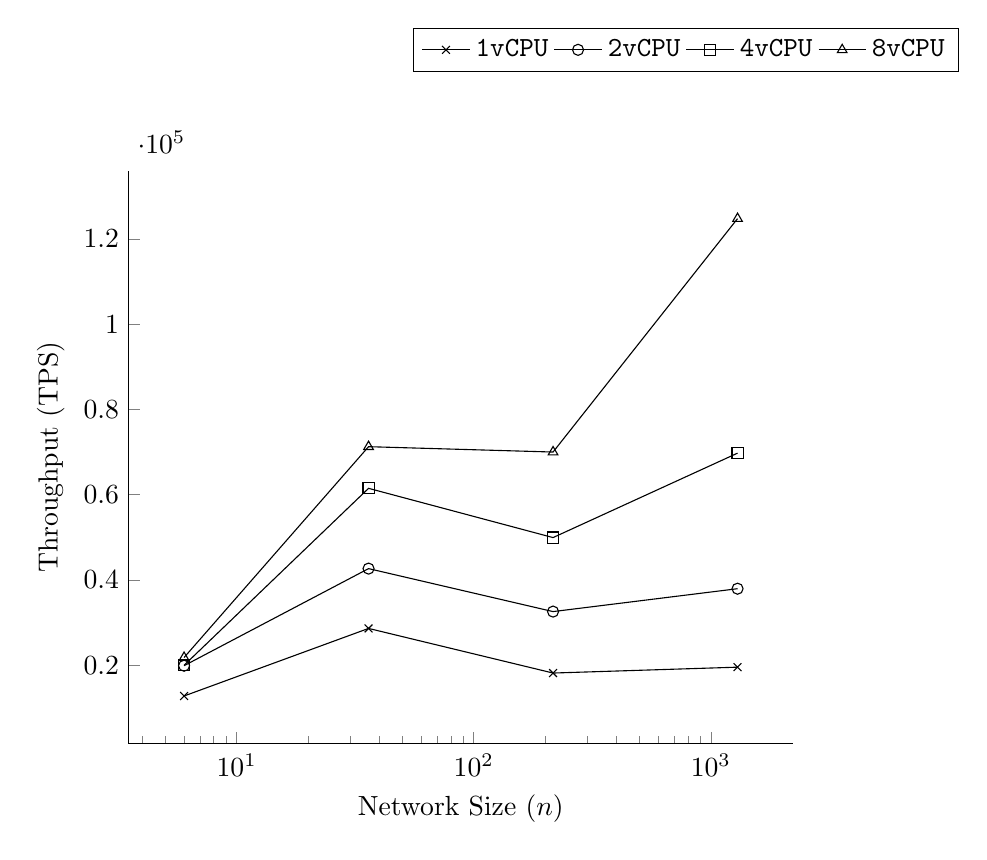
\begin{tikzpicture}
      \pgfplotsset{
          scale only axis,
          every axis legend/.append style={ at={(1.25,1.25)}, 
          legend columns = 0}
          % legend style={at={(0.5,0.5)},
      }
    
      \begin{axis}[
        xmode=log,
        %ymode=log,
        axis y line*=left,
        axis x line*=bottom,
        xlabel = Network Size ($n$),
        ylabel= Throughput (TPS),   
        scaled y ticks=true
      ]

        \addplot[mark=x,color=black] coordinates{
            (6,12757.6483092012)
            (36,28617)
            (216,18145.04)
            (1296,19524.42)
            % more points
          }; \label{plot_1_y1}
          
        \addplot[mark=o,color=black] coordinates{
            (6,19867.2694674749)
            (36,42655.0136745384)
            (216,32568.52)
            (1296,37939.67)
            % more points
          }; \label{plot_1_y2}
    
        \addplot[mark=square,color=black] coordinates{
            (6,19958.2378084842)
            (36,61495.6571839636)
            (216,49938.6)
            (1296,69754.93)	
            % more points
          }; \label{plot_1_y3}
          
        \addplot[mark=triangle,color=black] coordinates{
            (6,21786.3152948651)
            (36,71270.533771156)
            (216,70014.28)
            (1296,124795.86)	
            % more points
          }; \label{plot_1_y4}
        
        \addlegendimage{/pgfplots/refstyle=plot_1_y1}\addlegendentry{\texttt{1vCPU}}
        \addlegendimage{/pgfplots/refstyle=plot_1_y2}\addlegendentry{\texttt{2vCPU}}
        \addlegendimage{/pgfplots/refstyle=plot_1_y3}\addlegendentry{\texttt{4vCPU}}
        \addlegendimage{/pgfplots/refstyle=plot_1_y4}\addlegendentry{\texttt{8vCPU}}
        \end{axis}
    \end{tikzpicture}
    \caption{Average network throughput (TPS) at a given configuration (indicated above).}
    \label{fig:test_tps}
\end{figure}

% 	6	36	216	1296
% Throughput [1.vCPU] (TPS)	12757.6483092012	28617	18145.04	19524.42
% Throughput [2.vCPU] (TPS)	19867.2694674749	42655.0136745384	32568.52	37939.67
% Throughput [4.vCPU] (TPS)	19958.2378084842	61495.6571839636	49938.6	69754.93
% Throughput [8.vCPU] (TPS)	21786.3152948651	71270.533771156	70014.28	124795.86
\begin{figure}[h!]
    \centering
    \begin{tikzpicture}
      \pgfplotsset{
          scale only axis,
          every axis legend/.append style={ at={(1.25,1.25)}, 
          legend columns = 0}
          % legend style={at={(0.5,0.5)},
      }
    
      \begin{axis}[
        xmode=log,
        ymode=log,
        axis y line*=left,
        axis x line*=bottom,
        xlabel = Network Size ($n$),
        ylabel= Finality (Fin),   
        scaled y ticks=true
      ]

        \addplot[mark=x,color=black] coordinates{
            (6,0.455107294288512)
            (36,1.29)
            (216,10.95)
            (1296,59.08)
            % more points
          }; \label{plot_1_y1}
          
        \addplot[mark=o,color=black] coordinates{
            (6,0.27530306109322)
            (36,0.849044639878005)
            (216,5.44)
            (1296,26.64)
            % more points
          }; \label{plot_1_y2}
    
        \addplot[mark=square,color=black] coordinates{
            (6,0.274978588764595)
            (36,0.569285265953815)
            (216,2.68)
            (1296,10.59)	
            % more points
          }; \label{plot_1_y3}
          
        \addplot[mark=triangle,color=black] coordinates{
            (6,0.260436966149718)
            (36,0.489546359299769)
            (216,1.79)
            (1296,6.13)	
            % more points
          }; \label{plot_1_y4}
        
        \addlegendimage{/pgfplots/refstyle=plot_1_y1}\addlegendentry{\texttt{1vCPU}}
        \addlegendimage{/pgfplots/refstyle=plot_1_y2}\addlegendentry{\texttt{2vCPU}}
        \addlegendimage{/pgfplots/refstyle=plot_1_y3}\addlegendentry{\texttt{4vCPU}}
        \addlegendimage{/pgfplots/refstyle=plot_1_y4}\addlegendentry{\texttt{8vCPU}}
        \end{axis}
    \end{tikzpicture}
    \caption{Average network finality at a given configuration (indicated above).}
    \label{fig:test_fin}
\end{figure}

% 	6	36	216	1296
% Finality [1.vCPU]	0.455107294288512	1.29	10.95	59.08
% Finality [2.vCPU] 	0.27530306109322	0.849044639878005	5.44	26.64
% Finality [4.vCPU]	0.274978588764595	0.569285265953815	2.68	10.59
% Finality [8.vCPU]	0.260436966149718	0.489546359299769	1.79	6.13


\begin{figure}[h!]
    \centering
    \begin{tikzpicture}
      \pgfplotsset{
          scale only axis,
          every axis legend/.append style={ at={(1.25,1.25)}, 
          legend columns = 0}
          % legend style={at={(0.5,0.5)},
      }
    
      \begin{axis}[
        xmode=log,
        ymode=log,
        axis y line*=left,
        axis x line*=bottom,
        xlabel = Network Size ($n$),
        ylabel= Transactions (Tx) per Epoch,   
        scaled y ticks=true
      ]

        \addplot[mark=x,color=black] coordinates{
            (6,5919)
            (36,32531)
            (216,199719)
            (1296,1155692)
            % more points
          }; \label{plot_1_y1}
          
        \addplot[mark=o,color=black] coordinates{
            (6,5736)
            (36,33493)
            (216,177556)
            (1296,1015081)
            % more points
          }; \label{plot_1_y2}
    
        \addplot[mark=square,color=black] coordinates{
            (6,5830)
            (36,33133)
            (216,134270)
            (1296,741752)	
            % more points
          }; \label{plot_1_y3}
          
        \addplot[mark=triangle,color=black] coordinates{
            (6,5809)
            (36,34574)
            (216,126303)
            (1296,767379)	
            % more points
          }; \label{plot_1_y4}
        
        \addlegendimage{/pgfplots/refstyle=plot_1_y1}\addlegendentry{\texttt{1vCPU}}
        \addlegendimage{/pgfplots/refstyle=plot_1_y2}\addlegendentry{\texttt{2vCPU}}
        \addlegendimage{/pgfplots/refstyle=plot_1_y3}\addlegendentry{\texttt{4vCPU}}
        \addlegendimage{/pgfplots/refstyle=plot_1_y4}\addlegendentry{\texttt{8vCPU}}
        \end{axis}
    \end{tikzpicture}
    \caption{The average number of transactions in each epoch at a given configuration (indicated above), where each transaction is equivalent to 400 \texttt{bytes} of data (0.4\texttt{kB}).}
    \label{fig:test_tx}
\end{figure}

% 	6	36	216	1296
% Tx per Epoch [1.vCPU]	5919	32531	199719	1155692
% Tx per Epoch [2.vCPU]	5736	33493	177556	1015081
% Tx per Epoch [4.vCPU]	5830	33133	134270	741752
% Tx per Epoch [8.vCPU] 	5809	34574	126303	767379

\subsection{Discussion}\label{bench:dis}
The results from our testing, depicted in \textit{Figure} \ref{fig:test_tps}, \textit{Figure} \ref{fig:test_fin}, and \textit{Figure} \ref{fig:test_tx}, are closely aligned with our expectations going into the experiment, with rates of change in performance between \texttt{vCPU} thresholds (e.g. \texttt{1vCPU} to \texttt{2vCPU} to \texttt{4vCPU} to \texttt{8vCPU}) hitting some threshold at lower network sizes (6 nodes and 36 nodes), while changing at a near-linear rate for larger network sizes (216 nodes and 1,296 nodes). The reasons we expect for the observed \textit{near-linear} rates of change, especially at larger network sizes, is expected as a derivative of fluctuating epoch sizes, with \textit{transactions per Epoch} noticeably decreasing as the number of compute resources (\texttt{vCPU}) available to each node increase.

The reasons we believe to be the cause of the observed fluctuation in \textit{transactions per Epoch} are derived from the nature of the protocol. As Finality decreases in correlation with the increased availability of \texttt{vCPU's} per node, each node is required to collect the same block of transactions (ideally 1,000 transactions). With less time to complete the same task, while prioritizing the validation of an increasingly large number of transactions each epoch, we expect the likelihood each node fails to properly receive, validate, or batch client transactions to increase by a reasonable margin of error. While we do not observe the loss of any data as a consequence of this transaction process, with the distributed ledger at the end of each experiment maintaining the expected transactions, the number of epochs processed by the networks was larger than the ideal expectation across all network sizes. This is to be expected; however, further analysis to understand the rate of change across network sizes would be valuable in our process to understand the change in network performance across scales.

\subsection{Projection Modeling}\label{bench:mod}
When referencing the projections originally postulated in \textit{\nameref{proj:tps}} [\S\ref{proj:tps}], we found that our formulas were successful in their ability to project the performance of \textit{Blossom} within a reasonable margin of error. However, this correlation is highly dependent on the use of appropriate variables. In the scenario where incorrect variables are implemented, projected performance may drastically over-perform or under-perform the real-world outcome of the given node configuration. When referencing the testing completed in this section, the variables which accurately reflect the network configuration we implemented for our testing are as follows: \(\{
l = 335, \
v = 34700
\}\). All other variables will be updated in line with the configuration of the network simulation.

When assuming a constant utilization rate ($E$) across network scales, we may project the optimal performance of the network given the same benchmarks outlined in the previous figures (\textit{Figure} \ref{fig:test_tps}, \textit{Figure} \ref{fig:test_fin}, and \textit{Figure} \ref{fig:test_tx}). These projections can be observed in Figure 11.

\subsection{Comparisons}\label{bench:comp}
To substantiate the improvements we have displayed with our protocol, we are interested in equating our infrastructure to the performance of legitimate extant decentralized networks. Given the variance in node requirements for said networks, we determined it we be most appropriate to only reference the platforms which require comparable resources to those we may deploy during our testing. It is, for this reason, we have decided to exclude networks with excessive hardware requirements or the platforms which require the use of a \texttt{GPU} or \texttt{ASIC} processor (e.g. Bitcoin, Solana, Cosmos, Polygon, Stellar, etc…), with the platforms we measure against and their performance displayed in \textit{Table} \ref{tab:tab2}. While we are accepting the “claimed” performance results of these platforms for our comparison, we will be excluding the experimental result of most platforms as their testing is considered non-comparable, with the sole inclusion of Avalanche (noted as Ava Test).

\begin{table}[!h]
\centering
    \begin{tabular}{cccccc}
     \hline
     \textbf{Platform}& $n$ & \texttt{vCPU} &\texttt{RAM} &TPS&Fin (s)\\
     \hline
     Ethereum &5500 &4 &16 &30 &1,800\\
     Cardano &3200 &4 &16 &250 &1,200\\
     Algorand &1200 &16 &32 &6,000 &4\\
     Ava Test &2000 &2 &4 &3,401 &1.35\\
     Avalanche &1200 &8 &16 &4,500 &2\\
     \hline

    \end{tabular}
    \caption{The list of decentralized networks we believe as comparable given our testing results, as well as the estimated number of nodes (Nodes), the minimum CPU and RAM requirements to run a node (measured as equivalent AWS \texttt{vCPU’s}), as well as the TPS and Finality claimed by networks.}
    \label{tab:tab2}
\end{table}

As we have limited our testing (see \textit{\nameref{bench:res}} [\S\ref{bench:res}]) to specific network configurations which in most cases differ from the configuration of the precedent systems we have listed in \textit{Table} \ref{tab:tab2}, to undergo a one-to-one comparative analysis between \textit{Blossom} and each extant platform we will be referencing the protocols projected performance, utilizing the formula discussed in the previous section (\textit{\nameref{bench:mod}} [\S\ref{bench:mod}]). These comparisons will be made within reasonable confidence, calculated from the observed deviations of our performance, while implementing maximal utilization (see \textit{Table} \ref{tab:tab3}) and optimal utilization (see \textit{Table} \ref{tab:tab4}).

\begin{table}[h!]
\centering

    \begin{tabular}{cccccc}
     \hline
     \textbf{Platform}& TPS & Fin (s) &TPS $\%$ &Fin $\%$\\
     \hline
     Ethereum &103,691 &50.39 &345,638$\%$ &(97.20$\%$)\\
     Cardano &102,054 &29.79 &40,822$\%$ &(97.52$\%$)\\
     Algorand &305,971 &3.73 &5,100$\%$ &(6.75$\%$)\\
     Ava Test &52,168 &36.42 &1,534$\%$ &2,597.78$\%$\\
     Avalanche &179,054 &6.37 &3,979$\%$ &218.50$\%$\\
     \hline
    \end{tabular}
    \caption{The percentile performance difference between our platform, and the listed platform. TPS  — higher is better. Finality — lower is better.}
    \label{tab:tab3}
\end{table}

From the results in \textit{Table} \ref{tab:tab3} it is clear we have developed a competitive protocol, with immense increases in platform throughput, while finality remained within a reasonable margin of competing platforms in a majority of scenarios. The two (2) instances where our platform was outperformed, were both at the hands of Avalanche, with the finality of their platform occurring 4.37 seconds and 35.07 seconds faster than our protocol on comparable hardware. As our protocol has been tuned to optimize for throughput rather than finality, we do believe it reasonable that there exist cases where our platform is slower to reach finality than others. However, in cases where network utilization is reduced, the likelihood a \texttt{CPU} or bandwidth bottleneck may occur is drastically reduced. We experience the unique issue of network overutilization, as unlike other platforms we allow for parallel block insertion, with every node able to distribute a block of 1,000 transactions (\(\beta = 1000\)).

When referencing the two comparative experiments where we were outperformed, \textit{Avalanche} and \textit{Ava Test}, though \textit{Avalanche} does not incorporate ‘blocks,’ instead utilizing a DAG infrastructure allowing for the constant insertion of novel transactions, they reference running “10 client processes, each of which maintains 400 outstanding transactions at any given time” \cite{sekniqi2020avalanche}. Thus, the clients utilized in the \textit{Ava Test} distributed a total of 4,000 transactions at any given moment. When compared to our testing with \textit{Blossom}, we distribute \(\sim 2,000,000\) transactions each epoch (compared to \textit{Ava Test}) and \(\sim 1,200,000\) transactions each epoch (compared to \textit{Avalanche}). This drastic difference in testing, and as a consequence throughput, show the unique design decisions which allow for our platform to be increasingly scalable.

To address the disparity in finality, throughput, and network utilization between \textit{Blossom} and extant systems we can recompute the data displayed in \textit{Figure} \ref{fig:proj_large}, this time implementing the \textit{ideal utilization} ($U$) of \textit{Blossom} as described in \textit{\nameref{proj:dyn_ut}} [\S\ref{proj:dyn_ut}]. For a majority of cases, the primary benefit of decreased utilization comes with a proportional decrease in network finality, with minimal decreases in TPS for networks of increasing size. When finality is exceptionally high (see \textit{Ava Test} in \textit{Table} \ref{tab:tab3}) by strategically reducing utilization we can see immense reductions in finality, while throughput is decreased at a lesser rate (see \textit{Table} \ref{tab:tab4}). For \textit{Blossom} implementations where finality is prioritized over throughput, network arbiters may implement a reduced block size, or other methods, to artificially improve performance.

\begin{table}[!h]
\centering
    \begin{tabular}{cccc}
     \hline
     \textbf{Platform} &TPS $\%$ $\Delta$  &Fin $\%$ $\Delta$ &$U$\\
     \hline
    Ethereum &9.70$\%$ &(80.47$\%$)& 15.48$\%$ \\
    Cardano &0.20$\%$ &(78.01$\%$)& 22.32$\%$ \\
    Algorand &0.09$\%$ &(25.74$\%$)& 64.98$\%$ \\
    Ava Test &2.23$\%$ &(79.60$\%$)& 19.82$\%$ \\
    Avalanche &0.13$\%$ &(51.49$\%$)& 44.17$\%$ \\
     \hline
    \end{tabular}
    \caption{The percentile change in performance of the measurments collected in \textit{Table} \ref{tab:tab3} when operating at ideal utilization. TPS  — higher is better. Finality — lower is better.}
    \label{tab:tab4}
\end{table}

Referencing the new performance measurements displayed in \textit{Table} \ref{tab:tab4}, we can see that at \textit{ideal utilization} we are able to further reduce time to finality, without any meaningful change in network throughput. These results support the benefit of algorithmically modulating utilization rates to meet demand, as changes in utilization may provide increased performance. This is good for the competitiveness of \textit{Blossom}, allowing the protocol to be implemented for applications that are increasingly time-sensitive and requiring fast finality, guaranteeing the protocol is capable of maintaining performance, if not improving performance, given variations in network utilization.
